% ---------------------------------------------------------------------------
% Caderno 5 — Economia de ensaios e uso científico
% Compilação (MiKTeX fora do PATH):
%   $env:PATH = "C:\Users\Narcísius\AppData\Local\Programs\MiKTeX\miktex\bin\x64;" + $env:PATH
%   pdflatex -interaction=nonstopmode main.tex   (três vezes)
% ---------------------------------------------------------------------------
\documentclass{doeapostila}

% ---------------------------------------------------------------------------
% macros.tex — notação matemática comum aos cinco cadernos.
% Fixada antes de qualquer caderno começar, para os cinco não divergirem.
% Uso: % ---------------------------------------------------------------------------
% macros.tex — notação matemática comum aos cinco cadernos.
% Fixada antes de qualquer caderno começar, para os cinco não divergirem.
% Uso: % ---------------------------------------------------------------------------
% macros.tex — notação matemática comum aos cinco cadernos.
% Fixada antes de qualquer caderno começar, para os cinco não divergirem.
% Uso: \input{../estilo/macros} no preâmbulo de cada main.tex.
% ---------------------------------------------------------------------------

% Somas de quadrados
\newcommand{\SQT}{\mathrm{SQ}_{\mathrm{T}}}    % total
\newcommand{\SQR}{\mathrm{SQ}_{\mathrm{R}}}    % da regressão
\newcommand{\SQr}{\mathrm{SQ}_{\mathrm{r}}}    % residual
\newcommand{\SQfaj}{\mathrm{SQ}_{\mathrm{faj}}}% falta de ajuste
\newcommand{\SQep}{\mathrm{SQ}_{\mathrm{ep}}}  % erro puro

% Médias quadráticas: \MQ{R}, \MQ{r}, \MQ{faj}, \MQ{ep}
\newcommand{\MQ}[1]{\mathrm{MQ}_{\mathrm{#1}}}

% Coeficientes de determinação
\newcommand{\Rdois}{R^{2}}
\newcommand{\Rajus}{R^{2}_{\mathrm{aj}}}

% Efeitos: \efeito{1}, \efeito{12}
\newcommand{\efeito}[1]{E_{#1}}

% Álgebra matricial do ajuste por mínimos quadrados
\newcommand{\vetbeta}{\boldsymbol{\beta}}
\newcommand{\matX}{\mathbf{X}}
\newcommand{\vety}{\mathbf{y}}
 no preâmbulo de cada main.tex.
% ---------------------------------------------------------------------------

% Somas de quadrados
\newcommand{\SQT}{\mathrm{SQ}_{\mathrm{T}}}    % total
\newcommand{\SQR}{\mathrm{SQ}_{\mathrm{R}}}    % da regressão
\newcommand{\SQr}{\mathrm{SQ}_{\mathrm{r}}}    % residual
\newcommand{\SQfaj}{\mathrm{SQ}_{\mathrm{faj}}}% falta de ajuste
\newcommand{\SQep}{\mathrm{SQ}_{\mathrm{ep}}}  % erro puro

% Médias quadráticas: \MQ{R}, \MQ{r}, \MQ{faj}, \MQ{ep}
\newcommand{\MQ}[1]{\mathrm{MQ}_{\mathrm{#1}}}

% Coeficientes de determinação
\newcommand{\Rdois}{R^{2}}
\newcommand{\Rajus}{R^{2}_{\mathrm{aj}}}

% Efeitos: \efeito{1}, \efeito{12}
\newcommand{\efeito}[1]{E_{#1}}

% Álgebra matricial do ajuste por mínimos quadrados
\newcommand{\vetbeta}{\boldsymbol{\beta}}
\newcommand{\matX}{\mathbf{X}}
\newcommand{\vety}{\mathbf{y}}
 no preâmbulo de cada main.tex.
% ---------------------------------------------------------------------------

% Somas de quadrados
\newcommand{\SQT}{\mathrm{SQ}_{\mathrm{T}}}    % total
\newcommand{\SQR}{\mathrm{SQ}_{\mathrm{R}}}    % da regressão
\newcommand{\SQr}{\mathrm{SQ}_{\mathrm{r}}}    % residual
\newcommand{\SQfaj}{\mathrm{SQ}_{\mathrm{faj}}}% falta de ajuste
\newcommand{\SQep}{\mathrm{SQ}_{\mathrm{ep}}}  % erro puro

% Médias quadráticas: \MQ{R}, \MQ{r}, \MQ{faj}, \MQ{ep}
\newcommand{\MQ}[1]{\mathrm{MQ}_{\mathrm{#1}}}

% Coeficientes de determinação
\newcommand{\Rdois}{R^{2}}
\newcommand{\Rajus}{R^{2}_{\mathrm{aj}}}

% Efeitos: \efeito{1}, \efeito{12}
\newcommand{\efeito}[1]{E_{#1}}

% Álgebra matricial do ajuste por mínimos quadrados
\newcommand{\vetbeta}{\boldsymbol{\beta}}
\newcommand{\matX}{\mathbf{X}}
\newcommand{\vety}{\mathbf{y}}


\definecaderno{5}{Economia de ensaios e uso científico}

\begin{document}

\begin{center}
  {\large\bfseries Economia de ensaios e uso científico}\par\smallskip
  {\normalsize Caderno 5}\par\smallskip
  {\normalsize Murilo Miguel Narciso}\par\smallskip
  {\footnotesize Instituto Militar de Engenharia \textbullet{} \today}
\end{center}

\vspace{0.6\baselineskip}

\noindent
Os quatro cadernos anteriores tratam da construção do planejamento, da
estimação dos efeitos e da superfície de resposta. Este caderno fecha a série
tratando de uma restrição que os antecede na prática, o esforço experimental é
finito, e de uma consequência que os sucede, a forma como esse esforço é
relatado condiciona a credibilidade do que se publica. A primeira metade
apresenta o fatorial fracionado como resposta disciplinada à escassez de
ensaios, e não como atalho: fraciona-se apenas o que a hierarquia de efeitos
autoriza a sacrificar, e a projeção mostra que a aposta raramente é perdida
por completo. A segunda metade trata do orçamento de material como restrição
de projeto, do critério para encerrar uma campanha experimental e do que
declarar em um artigo para que o planejamento sustente, e não apenas
acompanhe, a alegação de rigor científico.

\vspace{0.6\baselineskip}

\tableofcontents

\section{O problema da escala}
\label{sec:escala}

O número de ensaios de um planejamento fatorial completo cresce de forma
exponencial com o número de fatores, enquanto o interesse prático do
pesquisador cresce apenas de forma linear, mais um fator relevante para
investigar, mais uma dimensão da malha experimental. Com sete fatores a dois
níveis, um fatorial completo exige $2^{7} = 128$ ensaios, número descrito na
literatura de referência como simplesmente inviável para a maioria dos
laboratórios.

A origem do crescimento fica evidente ao se decompor o total de ensaios pela
ordem das interações que ele permite estimar. Cada ensaio de um plano $2^{N_X}$
contribui para a estimação de $\binom{N_X}{i}$ efeitos de ordem $i$ (a média
sendo a ordem zero), e a soma de todos os $\binom{N_X}{i}$ ao longo de
$i = 0, \dots, N_X$ reproduz exatamente $2^{N_X}$, o total de ensaios. A
Tabela~\ref{tab:pascal} apresenta essa decomposição para $N_X$ de três a sete
fatores, que é a mesma leitura do triângulo de Pascal linha a linha.

\begin{table}[H]
  \centering
  \caption{Número de efeitos por ordem de interação em planejamentos $2^{N_X}$
    completos. Cada linha soma exatamente $2^{N_X}$, o número de ensaios do
    plano completo. Fonte: UFSC, \emph{Planejamento de Experimentos}, parte 5,
    p.~5.}
  \label{tab:pascal}
  \begin{tabular}{c S[table-format=1.0] S[table-format=1.0] S[table-format=2.0]
                    S[table-format=2.0] S[table-format=2.0] S[table-format=2.0]
                    S[table-format=1.0] S[table-format=3.0]}
    \toprule
    {$N_X$} & {ordem 0} & {ordem 1} & {ordem 2} & {ordem 3} & {ordem 4} &
      {ordem 5} & {ordem 6/7} & {total} \\
    \midrule
    3 & 1 & 3  & 3  & 1  & {--} & {--} & {--} & 8   \\
    4 & 1 & 4  & 6  & 4  & 1    & {--} & {--} & 16  \\
    5 & 1 & 5  & 10 & 10 & 5    & 1    & {--} & 32  \\
    6 & 1 & 6  & 15 & 20 & 15   & 6    & 1    & 64  \\
    7 & 1 & 7  & 21 & 35 & 35   & 21   & 7    & 128 \\
    \bottomrule
  \end{tabular}
\end{table}

A Figura~\ref{fig:ensaios-por-arranjo} traz a mesma progressão em escala
logarítmica, contrastando o fatorial completo com dois arranjos que este
caderno constrói nas seções seguintes, a meia-fração e o planejamento saturado
de resolução três. O contraste no extremo de sete fatores é o mais expressivo
do caderno, cento e vinte e oito ensaios contra apenas oito, e a linha
tracejada horizontal marca um orçamento hipotético de dezesseis corpos de
prova, quantidade insuficiente até para um fatorial completo de cinco
fatores.

\begin{figure}[H]
  \centering
  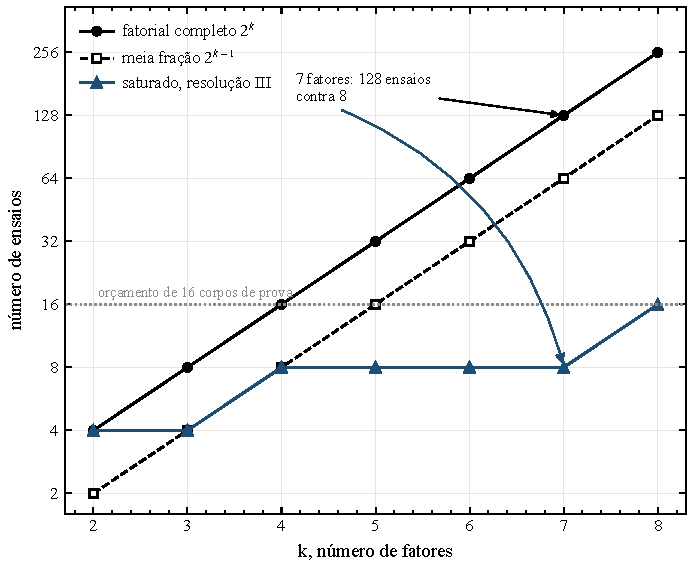
\includegraphics[width=0.82\linewidth]{../figuras/out/c5-ensaios-por-arranjo.pdf}
  \caption{Número de ensaios por arranjo, em escala logarítmica, para o
    fatorial completo $2^{k}$, a meia-fração $2^{k-1}$ e o planejamento
    saturado de resolução três. Fonte: UFSC, \emph{Planejamento de
    Experimentos}, parte 5, p.~4 a 5.}
  \label{fig:ensaios-por-arranjo}
\end{figure}

O restante deste caderno responde à pergunta que a Tabela~\ref{tab:pascal} e a
Figura~\ref{fig:ensaios-por-arranjo} deixam em aberto, quais dos $2^{N_X}-1$
efeitos além da média podem ser dispensados sem que a conclusão do
experimento fique comprometida, e o que fazer quando o orçamento não permite
sequer decidir isso com folga.

\begin{aplicacao}{A aritmética por trás de cento e vinte e oito ensaios}
  Para $N_X = 7$, a soma dos coeficientes binomiais da Tabela~\ref{tab:pascal}
  é $1 + 7 + 21 + 35 + 35 + 21 + 7 + 1 = 128$, confirmando por contagem direta
  o valor $2^{7}$. A Seção~\ref{sec:saturados} deste caderno retoma
  exatamente esses sete fatores e mostra como investigá-los com apenas oito
  ensaios, ao custo de aceitar confundimento entre efeitos.
\end{aplicacao}

\section{Hierarquia de efeitos}
\label{sec:hierarquia}

A viabilidade de qualquer fracionamento depende de uma regularidade empírica
observada em processos físicos e químicos, efeitos principais tendem a ser
maiores que interações de segunda ordem, que por sua vez tendem a ser maiores
que interações de terceira ordem, e assim sucessivamente. A razão intuitiva é
que uma interação de ordem alta exige a ação coordenada e simultânea de
muitos fatores sobre a resposta, condição progressivamente menos comum à
medida que a ordem cresce. Essa hierarquia não é uma lei, é uma tendência
observada com frequência suficiente para justificar, na prática, que
interações de ordem alta sejam tratadas como desprezíveis e que os graus de
liberdade que lhes seriam dedicados sejam redirecionados para reduzir o
número de ensaios.

O planejamento $2^{4}$ completo de \texttt{peixoto-2a4} ilustra a tendência
com dados reais. A Tabela~\ref{tab:hierarquia} agrupa os quinze efeitos não
triviais desse planejamento pela ordem da interação e reporta o intervalo de
magnitude, em valor absoluto, observado em cada grupo.

\begin{table}[H]
  \centering
  \caption{Magnitude dos efeitos do planejamento $2^{4}$ completo, agrupados
    por ordem de interação. Fonte: Peixoto, capítulo 4, p.~3 a 4.}
  \label{tab:hierarquia}
  \begin{tabular}{c c S[table-format=3.3] S[table-format=3.3]}
    \toprule
    Ordem & Número de efeitos & {Menor $|\efeito{}|$} & {Maior $|\efeito{}|$} \\
    \midrule
    1.\textsuperscript{a} (principal) & 4 & 2.375  & 109.375 \\
    2.\textsuperscript{a} (binária)   & 6 & 1.125  & 25.625  \\
    3.\textsuperscript{a} (ternária)  & 4 & 0.125  & 5.375   \\
    4.\textsuperscript{a} (quaternária) & 1 & \multicolumn{2}{c}{8.875} \\
    \bottomrule
  \end{tabular}
\end{table}

Os efeitos principais $\efeito{2} = \num{109.375}$, $\efeito{4} =
\num{67.125}$ e $\efeito{3} = \num{54.375}$ dominam o conjunto, enquanto as
três interações ternárias $\efeito{123}$, $\efeito{124}$ e $\efeito{234}$
ficam abaixo de \num{5.4} em módulo. A tendência, no entanto, não é absoluta,
a interação quaternária $\efeito{1234} = \num{-8.875}$ supera em módulo quatro
das seis interações binárias e todas as quatro interações ternárias. É
justamente por a hierarquia ser uma tendência, e não uma garantia, que a
projeção (Seção~\ref{sec:projecao}) e o dobramento (Seção~\ref{sec:dobramento})
existem como mecanismos de verificação a posteriori.

\begin{aplicacao}{Quando a hierarquia falha}
  Um planejamento que aliasse $\efeito{1234}$ a um efeito principal, como
  ocorre em planos de resolução mais baixa, herdaria integralmente essa
  interação quaternária na estimativa do efeito principal, uma contaminação
  de quase nove unidades, e a suposição de que interações de ordem alta são
  desprezíveis não bastaria para detectar o problema sem uma verificação
  independente.
\end{aplicacao}

\section{A meia-fração}
\label{sec:meia-fracao}

A meia-fração reduz o número de ensaios à metade ao reter apenas as
condições experimentais em que o produto de todos os sinais codificados dos
fatores é constante. Para um planejamento $2^{4}$, a fração definida pela
relação geradora $I = 1234$ mantém somente os ensaios em que
$z_{1}z_{2}z_{3}z_{4} = +1$, oito das dezesseis condições originais.

Aplicada ao conjunto \texttt{peixoto-2a4}, essa regra seleciona os ensaios 1,
4, 6, 7, 10, 11, 13 e 16. A Tabela~\ref{tab:meia-fracao} apresenta os efeitos
estimados a partir apenas desses oito ensaios, junto da combinação de efeitos
do fatorial completo que cada um deles estima.

\begin{table}[H]
  \centering
  \caption{Efeitos estimados na meia-fração $2^{4-1}$ com geratriz $I = 1234$
    (ensaios 1, 4, 6, 7, 10, 11, 13, 16 do fatorial completo). Fonte: Peixoto,
    capítulo 4, p.~5 a 8.}
  \label{tab:meia-fracao}
  \begin{tabular}{l S[table-format=3.3] l}
    \toprule
    Termo & {Valor} & Estima, no fatorial completo \\
    \midrule
    Média  & 138.875 & $M$ \\
    $e_{1}$  & -2.25   & $\efeito{1} + \efeito{234}$ \\
    $e_{2}$  & 114.75  & $\efeito{2} + \efeito{134}$ \\
    $e_{3}$  & 51.75   & $\efeito{3} + \efeito{124}$ \\
    $e_{4}$  & 69.75   & $\efeito{4} + \efeito{123}$ \\
    $e_{12}$ & 8.75    & $\efeito{12} + \efeito{34}$ \\
    $e_{13}$ & 24.75   & $\efeito{13} + \efeito{24}$ \\
    $e_{14}$ & 26.75   & $\efeito{14} + \efeito{23}$ \\
    \bottomrule
  \end{tabular}
\end{table}

A fração complementar, definida por $I = -1234$, retém os oito ensaios
restantes e fornece uma segunda estimativa independente da mesma combinação
de efeitos, com o sinal da interação de quarta ordem invertido. Combinando as
duas frações recupera-se a estimativa do fatorial completo, conforme a
Equação~\eqref{eq:recomposicao}:

\begin{equation}
  \frac{e_{i} + e_{i}^{*}}{2} = \efeito{i} .
  \label{eq:recomposicao}
\end{equation}

Na fração complementar, a média observada é \num{147.75} e o efeito
$e_{2}^{*} = \num{104.00}$. Combinando com $e_{2} = \num{114.75}$ da
Tabela~\ref{tab:meia-fracao}, obtém-se
$(\num{114.75} + \num{104.00})/2 = \num{109.375}$, valor idêntico ao efeito
$\efeito{2}$ do fatorial completo. O procedimento não é aproximado, é exato,
porque as duas frações juntas reconstituem todos os dezesseis ensaios
originais.

\begin{aplicacao}{Verificação da recomposição}
  A recomposição da Equação~\eqref{eq:recomposicao} aplicada ao efeito 2
  fornece $(\num{114.75} + \num{104.00})/2 = \num{109.375}$, exatamente o
  valor de $\efeito{2}$ tabulado para o fatorial $2^{4}$ completo. A
  concordância exata, e não aproximada, confirma que nenhuma informação é
  perdida quando as duas metades de um fatorial fracionado são conduzidas em
  conjunto, apenas redistribuída entre o efeito principal e sua interação
  aliada.
\end{aplicacao}

\section{Confundimento}
\label{sec:confundimento}

Toda coluna de sinais de um planejamento fatorial satisfaz $z_{i}^{2} = 1$
em cada ensaio, porque os níveis codificados valem $\pm 1$. Essa propriedade
permite obter o padrão de confundimento de uma fração por manipulação
algébrica direta da relação geradora. Multiplicando ambos os lados de
$I = 1234$ pela coluna 1, e usando $z_{1}^{2} = 1$, obtém-se
$1 \cdot I = 1 \cdot 1234 = (1 \cdot 1) \cdot 234 = 234$, de modo que o
contraste da coluna 1 estima, na verdade, $\efeito{1} + \efeito{234}$.
Repetindo o procedimento para a coluna do produto 1 e 2, tem-se
$12 \cdot I = (1 \cdot 1)(2 \cdot 2) \cdot 34 = 34$, mostrando que as duas
interações binárias 12 e 34 se confundem entre si.

A Tabela~\ref{tab:confundimento} lista o padrão completo de confundimento da
meia-fração $2^{4-1}_{\mathrm{IV}}$ com $I = 1234$, obtido por esse mesmo
procedimento aplicado a cada coluna.

\begin{table}[H]
  \centering
  \caption{Padrão de confundimento da meia-fração $2^{4-1}_{\mathrm{IV}}$ com
    geratriz $I = 1234$. Fonte: Peixoto, capítulo 4, p.~13.}
  \label{tab:confundimento}
  \begin{tabular}{c c}
    \toprule
    Coluna estimada & Confunde-se com \\
    \midrule
    1  & 234 \\
    2  & 134 \\
    3  & 124 \\
    4  & 123 \\
    12 & 34  \\
    13 & 24  \\
    14 & 23  \\
    \bottomrule
  \end{tabular}
\end{table}

O padrão da Tabela~\ref{tab:confundimento} evidencia a razão de a meia-fração
com essa geratriz específica ser preferível a outras possíveis, os quatro
efeitos principais se confundem apenas com interações ternárias, que a
hierarquia de efeitos (Seção~\ref{sec:hierarquia}) autoriza a supor pequenas,
enquanto as interações binárias se confundem apenas entre si, nunca com um
efeito principal.

\begin{aplicacao}{Álgebra do confundimento da coluna 3}
  Multiplicando a relação geradora pela coluna 3, obtém-se
  $3 \cdot I = 3 \cdot 1234 = (3 \cdot 3) \cdot 124 = 124$, confirmando a
  terceira linha da Tabela~\ref{tab:confundimento}, o contraste da coluna 3
  estima $\efeito{3} + \efeito{124}$, e não $\efeito{3}$ isoladamente.
\end{aplicacao}

\section{Resolução III, IV e V}
\label{sec:resolucao}

A resolução de um planejamento fracionado classifica a gravidade do
confundimento que ele introduz. Um plano de resolução III confunde efeitos
principais com interações de segunda ordem; um plano de resolução IV mantém
os efeitos principais livres de interações de segunda ordem, mas confunde
interações de segunda ordem entre si; um plano de resolução V mantém livres
tanto os efeitos principais quanto as interações de segunda ordem, que só se
confundem com interações de terceira ordem. A meia-fração $2^{4-1}$ da
Seção~\ref{sec:confundimento}, com efeitos principais confundidos apenas com
interações ternárias e interações binárias confundidas apenas entre si, é de
resolução IV.

O mesmo conjunto de dezesseis ensaios de \texttt{peixoto-2a4} admite outra
leitura instrutiva. Reinterpretado não como um $2^{4}$ completo, mas como uma
fração $2^{5-1}_{\mathrm{V}}$ de cinco fatores com geratriz $I = 12345$, a
antiga interação $\efeito{1234}$ passa a ser o contraste do quinto fator, e
as dez interações binárias se confundem par a par com as dez interações
ternárias remanescentes, listadas na Tabela~\ref{tab:resolucao-v}.

\begin{table}[H]
  \centering
  \caption{Padrão de confundimento de $2^{5-1}_{\mathrm{V}}$ com geratriz
    $I = 12345$, obtido reinterpretando os mesmos dezesseis ensaios de
    \texttt{peixoto-2a4}. Fonte: Peixoto, capítulo 4, p.~23 a 25.}
  \label{tab:resolucao-v}
  \begin{tabular}{c c c c}
    \toprule
    Par confundido & & Par confundido & \\
    \midrule
    12 = 345 & & 24 = 135 & \\
    13 = 245 & & 25 = 134 & \\
    14 = 235 & & 34 = 125 & \\
    15 = 234 & & 35 = 124 & \\
    23 = 145 & & 45 = 123 & \\
    \bottomrule
  \end{tabular}
\end{table}

O quinto fator, sob essa leitura, estima $e_{5} = \num{-8.88}$, valor
idêntico, a menos do arredondamento da fonte, ao $\efeito{1234} =
\num{-8.875}$ do fatorial completo original. Nenhum efeito principal e
nenhuma interação binária se confunde com outro do mesmo tipo, é exatamente a
definição de resolução V aplicada a um caso concreto.

\begin{aplicacao}{Três frações, três riscos distintos}
  O planejamento saturado de sete fatores em oito ensaios, apresentado na
  Seção~\ref{sec:saturados}, é de resolução III, cada efeito principal se
  confunde com três interações binárias. A meia-fração de quatro fatores da
  Seção~\ref{sec:meia-fracao} é de resolução IV, os efeitos principais ficam
  protegidos, ao custo de perder a interação binária individual. A
  reinterpretação de cinco fatores desta seção é de resolução V, tanto
  efeitos principais quanto interações binárias ficam protegidos. O preço da
  proteção crescente é sempre o mesmo, mais ensaios para o mesmo número de
  fatores.
\end{aplicacao}

\section{Projeção}
\label{sec:projecao}

Um fator que não afeta a resposta não desaparece do planejamento quando essa
irrelevância se confirma, ele devolve ensaios. A fração deixa de ser fração e
volta a ser um fatorial completo nos fatores restantes, com réplicas
genuínas de brinde nos casos em que os ensaios excedem o necessário para
saturar o fatorial menor. É o argumento mais forte a favor da triagem, mesmo
quando o fracionamento é feito às cegas, o custo de errar sobre um fator que
se revela importante é moderado, e o benefício de acertar sobre um fator que
se revela inerte é uma reestruturação favorável do próprio planejamento, não
apenas uma economia de tempo.

O caso mais simples é o de uma fração $2^{3-1}_{\mathrm{III}}$ com geratriz
$I = 123$, apresentada na Tabela~\ref{tab:projecao}.

\begin{table}[H]
  \centering
  \caption{Fração $2^{3-1}_{\mathrm{III}}$ com geratriz $I = 123$, quatro
    ensaios em um cubo de oito vértices. Fonte: Peixoto, capítulo 4, p.~28.}
  \label{tab:projecao}
  \begin{tabular}{c c c c}
    \toprule
    Ensaio & Fator 1 & Fator 2 & Fator 3 \\
    \midrule
    1 & $-$ & $-$ & $+$ \\
    2 & $+$ & $-$ & $-$ \\
    3 & $-$ & $+$ & $-$ \\
    4 & $+$ & $+$ & $+$ \\
    \bottomrule
  \end{tabular}
\end{table}

Se o fator 1 se revelar inerte, sua coluna é descartada e sobram os fatores 2
e 3. Lendo as duas colunas restantes da Tabela~\ref{tab:projecao}, o par
$(-,+)$, $(-,-)$, $(+,-)$ e $(+,+)$ aparece exatamente uma vez cada, um
fatorial $2^{2}$ completo, sem qualquer confundimento remanescente entre os
fatores 2 e 3. Se, além do fator 1, o fator 2 também se revelar inerte,
resta apenas o fator 3, que assume o nível $+1$ nos ensaios 1 e 4 e o nível
$-1$ nos ensaios 2 e 3, ou seja, duas réplicas genuínas em cada nível, de
onde passa a existir, pela primeira vez nessa fração, uma estimativa de erro
puro.

O mesmo raciocínio se generaliza para frações maiores. Na meia-fração
$2^{4-1}$ da Seção~\ref{sec:meia-fracao} (oito ensaios, resolução IV), a
eliminação de qualquer um dos quatro fatores por inércia projeta os oito
ensaios sobre os três fatores restantes como um fatorial $2^{3}$ completo e
sem aliasing algum, oito ensaios para oito combinações possíveis, verificado
diretamente sobre os ensaios 1, 4, 6, 7, 10, 11, 13 e 16. Se dois fatores se
revelarem inertes, os oito ensaios se projetam sobre os dois fatores
restantes como um fatorial $2^{2}$ completo com duas réplicas por
combinação. A fração nunca é desperdiçada quando a hierarquia de efeitos
(Seção~\ref{sec:hierarquia}) se confirma.

\begin{aplicacao}{Uma fração que nunca perde}
  Descartada a coluna do fator 4 na meia-fração de \texttt{peixoto-2a4}, os
  oito ensaios remanescentes cobrem as oito combinações de sinais dos
  fatores 1, 2 e 3 uma única vez cada, um fatorial $2^{3}$ completo, livre de
  qualquer confundimento, obtido ao custo de zero ensaios adicionais. A
  suposição de que o fator 4 seria dispensável, caso se confirmasse, não
  apenas preservaria a informação sobre os três fatores restantes, como a
  tornaria mais completa do que era dentro da fração original.
\end{aplicacao}

\section{Triagem e planos saturados}
\label{sec:saturados}

Um planejamento é dito saturado quando o número de fatores estudados se
aproxima do máximo permitido pelo número de ensaios, deixando o mínimo de
graus de liberdade disponível para qualquer outra estimativa. O exemplo
canônico investiga sete fatores em apenas oito ensaios, um planejamento
$2^{7-4}_{\mathrm{III}}$ construído a partir de um fatorial $2^{3}$ completo
nos fatores 1, 2 e 3, ao qual se somam quatro colunas adicionais definidas
pelas relações $4 = 12$, $5 = 13$, $6 = 23$ e $7 = 123$. A Tabela~\ref{tab:saturado-fracao}
reproduz os oito ensaios e a resposta observada, conversão percentual de um
processo químico.

\begin{table}[H]
  \centering
  \caption{Planejamento saturado $2^{7-4}_{\mathrm{III}}$, sete fatores em
    oito ensaios. Fonte: Peixoto, capítulo 4, p.~34 a 36.}
  \label{tab:saturado-fracao}
  \footnotesize
  \begin{tabular}{c c c c c c c c S[table-format=2.0]}
    \toprule
    Ensaio & 1 & 2 & 3 & 4=12 & 5=13 & 6=23 & 7=123 & {$y$ (\%)} \\
    \midrule
    1 & $-$ & $-$ & $-$ & $+$ & $+$ & $+$ & $-$ & 56 \\
    2 & $+$ & $-$ & $-$ & $-$ & $-$ & $+$ & $+$ & 66 \\
    3 & $-$ & $+$ & $-$ & $-$ & $+$ & $-$ & $+$ & 51 \\
    4 & $+$ & $+$ & $-$ & $+$ & $-$ & $-$ & $-$ & 52 \\
    5 & $-$ & $-$ & $+$ & $+$ & $-$ & $-$ & $+$ & 54 \\
    6 & $+$ & $-$ & $+$ & $-$ & $+$ & $-$ & $-$ & 70 \\
    7 & $-$ & $+$ & $+$ & $-$ & $-$ & $+$ & $-$ & 42 \\
    8 & $+$ & $+$ & $+$ & $+$ & $+$ & $+$ & $+$ & 64 \\
    \bottomrule
  \end{tabular}
\end{table}

Nesse arranjo, cada contraste estimado a partir dos oito ensaios engloba, no
fatorial $2^{7}$ completo, dezesseis dos cento e vinte e oito efeitos
possíveis, contando a média, $128/8 = 16$, de modo que cada efeito individual
se confunde com outros quinze. Restringindo a leitura às interações de até
segunda ordem, por força da hierarquia de efeitos, cada contraste $e_{i}$
estima o efeito principal correspondente somado a três interações binárias
específicas, listadas na Tabela~\ref{tab:saturado-efeitos}.

\begin{table}[H]
  \centering
  \caption{Efeitos preliminares do planejamento saturado, antes do
    desconfundimento. Fonte: Peixoto, capítulo 4, p.~37.}
  \label{tab:saturado-efeitos}
  \begin{tabular}{c S[table-format=2.2] l}
    \toprule
    Contraste & {Valor} & Estima \\
    \midrule
    $e_{1}$ & 12.25 & $\efeito{1} + \efeito{24} + \efeito{35} + \efeito{67}$ \\
    $e_{2}$ & -9.25 & $\efeito{2} + \efeito{14} + \efeito{36} + \efeito{57}$ \\
    $e_{3}$ & 1.25  & $\efeito{3} + \efeito{15} + \efeito{26} + \efeito{47}$ \\
    $e_{4}$ & -0.75 & $\efeito{4} + \efeito{12} + \efeito{56} + \efeito{37}$ \\
    $e_{5}$ & 6.75  & $\efeito{5} + \efeito{13} + \efeito{46} + \efeito{27}$ \\
    $e_{6}$ & 0.25  & $\efeito{6} + \efeito{23} + \efeito{45} + \efeito{17}$ \\
    $e_{7}$ & 3.75  & $\efeito{7} + \efeito{34} + \efeito{25} + \efeito{16}$ \\
    \bottomrule
  \end{tabular}
\end{table}

Os contrastes $e_{1}$, $e_{2}$ e $e_{5}$ se destacam em magnitude, ao passo
que $e_{3}$, $e_{4}$ e $e_{6}$ ficam próximos de zero. O contraste $e_{7} =
\num{3.75}$ ocupa uma posição intermediária, e é justamente sobre um dos
efeitos combinados em $e_{5}$ que a ambiguidade se concentra, a interação
$\efeito{27}$ participa tanto de $e_{5}$ quanto, isoladamente, de nenhum
outro contraste isolável nesta fração, o que motiva o desconfundimento
apresentado na próxima seção.

\begin{aplicacao}{Um efeito por ensaio, quinze escondidos atrás dele}
  Com oito ensaios e cento e vinte e oito efeitos possíveis no fatorial
  completo de sete fatores, a fração saturada estima apenas oito contrastes
  independentes, a média e sete combinações lineares. Cada uma dessas
  combinações reúne dezesseis efeitos do fatorial completo, dos quais só os
  quatro de ordem até dois (o principal e três binários) recebem leitura
  neste caderno, por força da hierarquia de efeitos.
\end{aplicacao}

\section{Dobramento}
\label{sec:dobramento}

Desconfundir um efeito suspeito não exige descartar os ensaios já realizados
e recomeçar com um planejamento maior. Quando a análise preliminar da
Seção~\ref{sec:saturados} deixa dúvida sobre se o contraste $e_{5}$ reflete
principalmente o efeito 5 ou a interação $\efeito{27}$, uma segunda fração
menor, com apenas o sinal da coluna 5 invertido ($5^{*} = -13$, mantidas as
demais relações $4 = 12$, $6 = 23$ e $7 = 123$), basta para isolar a dúvida.

Definindo $s_{i} = (e_{i} + e_{i}^{*})/2$ e $d_{i} = (e_{i} - e_{i}^{*})/2$
a partir dos contrastes da fração original e da fração invertida, a soma
$s_{i}$ isola a parte do contraste que não depende do sinal de $5$, enquanto
a diferença $d_{i}$ isola exatamente a parte que depende. A
Tabela~\ref{tab:dobramento} apresenta o resultado completo.

\begin{table}[H]
  \centering
  \caption{Desconfundimento por inversão do sinal da coluna 5. Fonte:
    Peixoto, capítulo 4, p.~39 a 41.}
  \label{tab:dobramento}
  \footnotesize
  \begin{tabular}{c S[table-format=2.2] S[table-format=2.2] l l}
    \toprule
    $i$ & {$s_{i}$} & {$d_{i}$} & $s_{i}$ estima & $d_{i}$ estima \\
    \midrule
    1 & 12.75 & -0.50 & $\efeito{1}+\efeito{24}+\efeito{67}$ & $\efeito{35}$ \\
    2 & -7.00 & -2.25 & $\efeito{2}+\efeito{14}+\efeito{36}$ & $\efeito{57}$ \\
    3 & -0.25 & 1.50  & $\efeito{3}+\efeito{26}+\efeito{47}$ & $\efeito{15}$ \\
    4 & -1.25 & 0.50  & $\efeito{4}+\efeito{12}+\efeito{37}$ & $\efeito{56}$ \\
    5 & 4.75  & 2.00  & $\efeito{5}$                          & $\efeito{13}+\efeito{46}+\efeito{27}$ \\
    6 & 1.75  & -1.50 & $\efeito{6}+\efeito{23}+\efeito{17}$ & $\efeito{45}$ \\
    7 & 4.00  & -0.25 & $\efeito{7}+\efeito{34}+\efeito{16}$ & $\efeito{25}$ \\
    \bottomrule
  \end{tabular}
\end{table}

O desconfundimento isola $\efeito{5}$ dos demais termos que o acompanhavam em
$e_{5}$, o valor $s_{5} = \num{4.75}$ responde por \num{4.75} dos \num{6.75}
pontos percentuais originalmente atribuídos ao conjunto
$\efeito{5}+\efeito{13}+\efeito{46}+\efeito{27}$, restando apenas \num{2.00}
pontos para as três interações binárias combinadas, que se confirmam pouco
relevantes. O erro do contraste, estimado a partir dos sete valores de
$d_{i}$ por $S_{C} = \sqrt{\sum d_{i}^{2}/7}$, vale $\num{1.42}$, valor usado
para construir os intervalos de confiança finais da
Tabela~\ref{tab:intervalos-saturado}.

\begin{table}[H]
  \centering
  \caption{Intervalos de 95\% de confiança dos sete efeitos do planejamento
    saturado, com $t^{*} = 2.776$. Fonte: Peixoto, capítulo 4, p.~42, versão
    corrigida (ver nota de rodapé).}
  \label{tab:intervalos-saturado}
  \begin{tabular}{c S[table-format=-2.2] S[table-format=2.2] c}
    \toprule
    Efeito & {Limite inferior} & {Limite superior} & Contém zero? \\
    \midrule
    $\efeito{1}$ & 8.31  & 16.19 & não, significativo \\
    $\efeito{2}$ & -13.19 & -5.31 & não, significativo \\
    $\efeito{3}$ & -2.69 & 5.19  & sim \\
    $\efeito{4}$ & -4.69 & 3.19  & sim \\
    $\efeito{5}$ & 2.81  & 10.69 & não, significativo \\
    $\efeito{6}$ & -3.69 & 4.19  & sim \\
    $\efeito{7}$\footnotemark & -0.19 & 7.69  & sim \\
    \bottomrule
  \end{tabular}
\end{table}
\footnotetext{A fonte original imprime o limite inferior do intervalo de
  $\efeito{7}$ como $0{,}2$, sem o sinal de menos. O valor correto, recalculado
  a partir dos mesmos $\hat{E}_{7}$ e $S_{C}$ impressos na própria fonte, é
  $-0{,}19$. Com o sinal correto o intervalo contém zero e $\efeito{7}$ deixa
  de ser significativo, permanecendo como efeitos relevantes apenas
  $\efeito{1}$, $\efeito{2}$ e $\efeito{5}$.}

Quando mais de um efeito precisa de desconfundimento simultâneo, o mesmo
princípio se generaliza ao dobramento completo do planejamento, invertendo o
sinal de todos os fatores de base e conduzindo o conjunto espelhado como um
segundo bloco de oito ensaios. O planejamento resultante, com dezesseis
ensaios ao todo, sobe de resolução III para IV, sem que os oito ensaios
originais sejam descartados.

\begin{aplicacao}{Dezesseis ensaios em vez de trinta e dois}
  Confirmar isoladamente a suspeita sobre $\efeito{5}$ custou apenas mais
  oito ensaios, com a coluna 5 invertida, e não os vinte e quatro ensaios
  adicionais que separariam completamente todas as interações binárias do
  planejamento. O dobramento resolve a dúvida específica que motivou sua
  execução, sem pretender resolver dúvidas que ninguém levantou.
\end{aplicacao}

\section{Orçamento de material}
\label{sec:orcamento}

Em pesquisas experimentais com materiais de origem natural, o número de
ensaios não é necessariamente uma escolha do pesquisador, pode ser uma
restrição imposta pela quantidade de material disponível. No estudo de
compósitos solo-fibra-cimento conduzido pelo autor deste caderno, a fibra
vegetal utilizada como reforço foi obtida em Manaus e transportada por via
aérea em quantidade limitada pela bagagem permitida. Cada corpo de prova
consome uma massa fixa de fibra, e a quantidade total disponível determina,
antes de qualquer consideração estatística, o número máximo de corpos de
prova que podem ser moldados. O planejamento experimental, nessas condições,
não escolhe o número de ensaios livremente, ele distribui um número de
ensaios já determinado pelo estoque de material entre os fatores e níveis
que mais interessa investigar.

A Tabela~\ref{tab:orcamento-material} sintetiza quantos corpos de prova cada
arranjo consome, para dois e três fatores, com e sem réplica, com e sem
pontos centrais, a partir da relação $N_{E} = N_{R} \cdot N_{L}^{N_X} +
N_{C0}$, em que $N_R$ é o número de réplicas por condição, $N_L$ o número de
níveis por fator e $N_{C0}$ o número de pontos centrais.

\begin{table}[H]
  \centering
  \caption{Corpos de prova consumidos por arranjo, para dois e três fatores a
    dois níveis. A meia-fração de dois fatores não é praticada, porque
    confundiria os dois efeitos principais entre si.}
  \label{tab:orcamento-material}
  \begin{tabular}{l c c c S[table-format=2.0]}
    \toprule
    Arranjo & $N_X$ & $N_R$ & Pontos centrais & {$N_E$} \\
    \midrule
    Fatorial completo                    & 2 & 1 & 0 & 4  \\
    Fatorial completo, replicado         & 2 & 2 & 0 & 8  \\
    Fatorial completo, com centrais      & 2 & 1 & 3 & 7  \\
    Fatorial completo, replicado, com centrais & 2 & 2 & 3 & 11 \\
    \midrule
    Fatorial completo                    & 3 & 1 & 0 & 8  \\
    Fatorial completo, replicado         & 3 & 2 & 0 & 16 \\
    Fatorial completo, com centrais      & 3 & 1 & 3 & 11 \\
    Fatorial completo, replicado, com centrais & 3 & 2 & 3 & 19 \\
    Meia-fração                          & 3 & 1 & 0 & 4  \\
    Meia-fração, replicada               & 3 & 2 & 0 & 8  \\
    Meia-fração, com centrais            & 3 & 1 & 3 & 7  \\
    Meia-fração, replicada, com centrais & 3 & 2 & 3 & 11 \\
    \bottomrule
  \end{tabular}
\end{table}

A Figura~\ref{fig:corpos-de-prova} traduz essa mesma restrição em termos de
capacidade de investigação. O painel (a) mostra quantos fatores um
planejamento saturado, um fatorial completo e um fatorial completo replicado
duas vezes conseguem investigar para diferentes tamanhos de orçamento de
corpos de prova, e o painel (b) mostra o preço, em graus de liberdade
disponíveis para estimar o erro, de espremer mais fatores nos mesmos
dezesseis ensaios.

\begin{figure}[H]
  \centering
  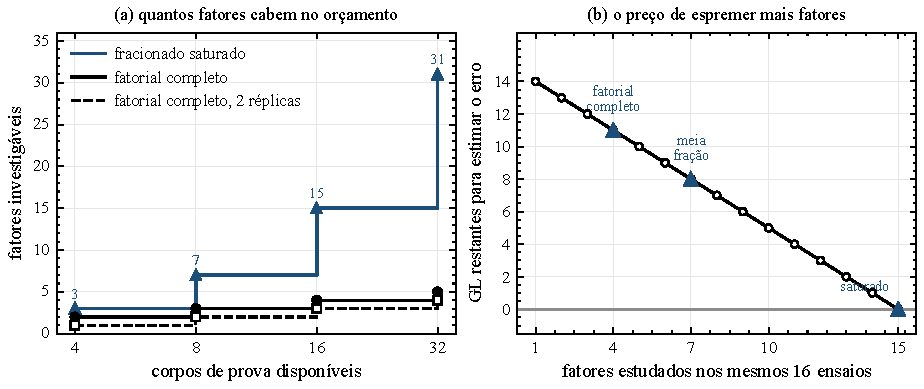
\includegraphics[width=0.95\linewidth]{../figuras/out/c5-corpos-de-prova-vs-informacao.pdf}
  \caption{Corpos de prova disponíveis contra informação extraída. Painel (a):
    fatores investigáveis por orçamento de corpos de prova. Painel (b): graus
    de liberdade restantes para estimar o erro, ao se estudarem cada vez mais
    fatores nos mesmos dezesseis ensaios.}
  \label{fig:corpos-de-prova}
\end{figure}

Com um orçamento de dezesseis corpos de prova, o painel (a) mostra que um
fatorial completo permite investigar quatro fatores, o mesmo fatorial
replicado duas vezes permite investigar apenas três, e um planejamento
fracionado saturado permite investigar até quinze. O painel (b) traduz o
mesmo custo de outra forma, ao subir de quatro para sete e depois para quinze
fatores nos mesmos dezesseis ensaios, os graus de liberdade disponíveis para
estimar o erro puro caem de onze para oito e depois para zero.

O trade-off é, portanto, explícito. Com um orçamento fixo de material,
fracionar permite investigar mais fatores, com menos confiança em cada um,
porque menos ensaios sobram para estimar o erro e desfazer confundimentos;
replicar permite investigar menos fatores, com mais confiança em cada um,
porque cada estimativa é sustentada por uma estimativa de erro puro genuína.
A escolha correta depende do estágio da investigação, não é uma preferência
fixa. No início de uma linha de pesquisa, quando muitos fatores candidatos
ainda não tiveram sua relevância confirmada, a triagem fracionada satura o
orçamento em largura, aceitando confundimento em troca de cobertura. Depois
que a triagem reduz a lista a poucos fatores relevantes, a etapa de
otimização satura o mesmo orçamento em profundidade, trocando cobertura por
réplicas e pontos centrais que sustentam um modelo de superfície de resposta
confiável.

\begin{aplicacao}{O mesmo estoque de fibra, duas estratégias}
  Um estoque de fibra vegetal suficiente para dezesseis corpos de prova
  permite, seguindo a Figura~\ref{fig:corpos-de-prova}, uma triagem saturada
  de até quinze fatores candidatos, como o tipo de fibra, o comprimento, o
  teor de cimento, o teor de água, o tempo de cura, entre outros, ou um
  estudo replicado e com pontos centrais de apenas três fatores já
  selecionados por triagem anterior. As duas opções consomem o mesmo
  material, respondem a perguntas de natureza diferente e nenhuma é
  substituta da outra.
\end{aplicacao}

\section{Quando parar}
\label{sec:quando-parar}

Uma campanha experimental pode ser encerrada quando o modelo ajustado
alcança o teto de variação explicável imposto pelo próprio ruído dos dados,
e não antes disso. Esse teto é dado por
$(\SQT - \SQep)/\SQT$, a fração da variação total que restaria explicada
mesmo por um modelo perfeito, e é determinado inteiramente pelas réplicas,
não pela forma funcional adotada. Exigir de um modelo um $\Rdois$ superior a
esse teto é exigir o impossível, a diferença remanescente é erro
experimental, não falta de ajuste.

O conjunto \texttt{peixoto-lin-quad} ilustra esse critério com precisão. Com
$\SQT = 8930$ e $\SQep = 45$, o teto de variação explicável vale
$\num{0.994961}$. O modelo quadrático ajustado a esses dados alcança
$\Rdois = \num{0.993461}$, a apenas \num{0.0015} do teto, uma diferença
pequena o suficiente para não justificar a inclusão de termos adicionais.
Confirma essa leitura o teste de falta de ajuste, $\MQ{faj}/\MQ{ep} =
\num{0.447}$, muito abaixo de qualquer limiar crítico usual.

Além do teto de $\Rdois$, três outros critérios encerram uma campanha
experimental de modo defensável. Primeiro, quando os intervalos de confiança
dos efeitos relevantes já são estreitos o suficiente para sustentar a
decisão prática que motivou o experimento, ampliá-los mais não muda a
conclusão. Segundo, quando os diagnósticos de resíduo não revelam estrutura
remanescente, nem tendência contra a ordem de execução, nem padrão contra o
valor ajustado, um modelo cujos resíduos já se comportam como ruído aleatório
não é melhorado por mais ensaios sob a mesma forma funcional. Terceiro,
quando o ganho marginal esperado de um novo ensaio, em redução de incerteza,
é inferior ao seu custo, seja esse custo material, como no orçamento da
Seção~\ref{sec:orcamento}, seja de tempo de laboratório.

\begin{aplicacao}{Um modelo já no teto}
  A diferença de apenas \num{0.0015} entre o $\Rdois$ do modelo quadrático de
  \texttt{peixoto-lin-quad} e o teto imposto pelo erro puro indica que
  qualquer termo adicional, cúbico ou de interação, estaria ajustando ruído,
  não sinal. A campanha experimental que produziu esses dezoito ensaios
  estava, nesse ponto, madura para encerramento.
\end{aplicacao}

\section{O planejamento de experimentos no artigo}
\label{sec:artigo}

A seção de materiais e métodos de um artigo científico que reporta um
experimento planejado precisa declarar quatro elementos para que o leitor
possa avaliar a validade da inferência, o arranjo adotado, com seus fatores,
níveis e eventual fracionamento e resolução, o número de réplicas por
condição, a existência ou ausência de blocos e o critério que os define, e a
ordem de execução dos ensaios, com a afirmação explícita de que foi sorteada
e não conduzida na sequência mais conveniente para o experimentador. A
omissão de qualquer um desses quatro pontos impede o leitor de distinguir um
efeito real de um artefato de condução.

Na seção de resultados, quatro elementos sustentam a mesma avaliação, a
tabela de análise de variância completa, com soma de quadrados, graus de
liberdade, quadrado médio, estatística $F$ e valor-p de cada termo, o
coeficiente de determinação $\Rdois$ acompanhado do seu ajustado $\Rajus$, os
valores-p de cada termo do modelo, não apenas do modelo como um todo, e os
gráficos de diagnóstico dos resíduos. A Tabela~\ref{tab:anova-artigo}
exemplifica o nível de detalhe esperado, reproduzindo a análise de variância
de uma composição central em dois blocos.

\begin{table}[H]
  \centering
  \caption{Exemplo do detalhamento esperado em uma tabela de análise de
    variância de artigo, composição central de dois fatores em dois blocos.
    Fonte: \texttt{origin-ccd}.}
  \label{tab:anova-artigo}
  \begin{tabular}{l S[table-format=3.3] c S[table-format=2.5]
                    S[table-format=1.5] S[table-format=1.5]}
    \toprule
    Fonte & {SQ} & GL & {MQ} & {$F$} & {$p$} \\
    \midrule
    Blocos          & 8.642857   & 1 & 8.642857  & 0.21681 & {--} \\
    Fibra           & 196.28731  & 1 & 196.28731 & 4.92385 & {--} \\
    Cimento         & 123.92399  & 1 & 123.92399 & 3.10862 & {--} \\
    Falta de ajuste & 361.3125   & 6 & 60.21875  & 6.45201 & 0.04628 \\
    Erro puro       & 37.33333   & 4 & 9.33333   & {--}    & {--} \\
    \bottomrule
  \end{tabular}
\end{table}

Reportar apenas $\Rdois$ é insuficiente, e o par $\Rdois = \num{0.34312}$ com
$\Rajus = \num{0.08037}$ do conjunto \texttt{origin-2x2} ilustra o motivo, um
$\Rdois$ modesto já sugere pouco poder explicativo, mas é o colapso do
ajustado, que penaliza a perda de graus de liberdade, que expõe um modelo
sem sustentação real. Omitir $\Rajus$ de um artigo priva o leitor exatamente
da informação que distingue um modelo genuíno de um modelo inflado por
termos supérfluos.

A prática de variar um fator de cada vez, mantendo os demais fixos,
enfraquece a revisão por pares porque impede a estimação de qualquer
interação, e a ausência de estimativa não significa ausência de interação,
apenas ausência de informação sobre ela. Um revisor que reconheça a técnica
não tem como avaliar se a conclusão reportada permaneceria válida fora das
condições fixas escolhidas, e a alegação de que um fator não interage com os
demais, quando não sustentada por um planejamento fatorial, é uma afirmação
não testada, apresentada como se fosse resultado.

A réplica e a aleatorização sustentam a alegação de reprodutibilidade por
caminhos distintos e complementares. A réplica fornece a estimativa de erro
puro contra a qual qualquer diferença observada é julgada, sem ela não existe
critério quantitativo para distinguir um efeito real de uma flutuação, e a
alegação de reprodutibilidade fica sem lastro numérico. A aleatorização, por
sua vez, protege contra fatores de perturbação não controlados que variam ao
longo do tempo de execução, garantindo que essas perturbações se distribuam
como ruído entre as condições experimentais, e não se acumulem
sistematicamente a favor ou contra alguma delas. Um experimento com réplicas
mas sem aleatorização pode ter erro puro corretamente estimado e ainda assim
efeitos sistematicamente viesados; a comparação dos cinco pares arma-radar,
com e sem reconhecimento do fabricante como bloco, ilustra como a mesma
réplica pode sustentar conclusões opostas conforme a ordem e o agrupamento
dos ensaios sejam ou não controlados.

\begin{aplicacao}{Um parágrafo de materiais e métodos}
  Adotou-se uma composição central rotacionável de dois fatores em dois
  blocos, com três pontos centrais por bloco, totalizando quatorze ensaios.
  A ordem de execução dos ensaios foi sorteada dentro de cada bloco. O teste
  de falta de ajuste indicou insuficiência do modelo linear
  ($F = \num{6.45201}$, $p = \num{0.04628}$), o que motivou a inclusão de
  termos quadráticos na etapa seguinte da investigação. Um parágrafo desse
  formato, com número, ordem e teste explicitados, permite que qualquer
  revisor reproduza o julgamento estatístico a partir dos números
  reportados, sem precisar confiar apenas na conclusão do autor.
\end{aplicacao}

\section{Exemplo de aplicação}
\label{sec:exemplo-final}

O planejamento $2^{3}$ completo do conjunto \texttt{peixoto-2x3} investiga
temperatura, catalisador e concentração de reagente com duas réplicas por
condição, dezesseis ensaios ao todo, e conclui que a concentração é
relevante mas não interage de forma importante com os demais fatores. Esta
seção reconstrói o mesmo estudo como se apenas oito ensaios estivessem
disponíveis, a meia-fração com geratriz $I = 123$ que mantém as quatro
condições em que $z_{1}z_{2}z_{3} = +1$, e convida o leitor a avaliar, antes
de ver a resposta completa, se a mesma conclusão seria alcançável com metade
do orçamento.

A Tabela~\ref{tab:exercicio-meia-fracao} apresenta as quatro condições
retidas por essa fração e as respectivas médias observadas.

\begin{table}[H]
  \centering
  \caption{Meia-fração $2^{3-1}$ de \texttt{peixoto-2x3}, com $I = 123$, quatro
    das oito condições do fatorial completo.}
  \label{tab:exercicio-meia-fracao}
  \begin{tabular}{c c c c S[table-format=2.1]}
    \toprule
    Condição & Temperatura & Catalisador & Concentração & {Resposta média} \\
    \midrule
    $(+,-,-)$ & 333 K & A & 1.0 M & 86.5 \\
    $(-,+,-)$ & 313 K & B & 1.0 M & 48.0 \\
    $(-,-,+)$ & 313 K & A & 1.5 M & 63.0 \\
    $(+,+,+)$ & 333 K & B & 1.5 M & 72.0 \\
    \bottomrule
  \end{tabular}
\end{table}

A partir apenas dessas quatro médias, os contrastes usuais de um fatorial
$2^{2}$ nos fatores livres temperatura e catalisador fornecem
$e_{T} = \num{23.75}$, $e_{\mathrm{Cat}} = \num{-14.75}$ e um terceiro
contraste, associado à coluna do produto temperatura vezes catalisador,
$e_{12} = \num{0.25}$.

\begin{aplicacao}{Gabarito do exercício de triagem}
  O fatorial completo, já conhecido integralmente, permite decompor cada
  contraste da meia-fração em sua combinação exata de efeitos aliados,
  $e_{T} = \efeito{T} + \efeito{\mathrm{Cat}\cdot\mathrm{Conc}} =
  \num{22.875} + \num{0.875} = \num{23.75}$, e
  $e_{\mathrm{Cat}} = \efeito{\mathrm{Cat}} + \efeito{T\cdot\mathrm{Conc}} =
  \num{-13.875} + \num{-0.875} = \num{-14.75}$, ambos confirmados
  exatamente. O terceiro contraste, no entanto, expõe o risco do
  fracionamento de resolução III, $e_{12} = \efeito{T\cdot\mathrm{Cat}} +
  \efeito{\mathrm{Conc}} = \num{-8.625} + \num{8.875} = \num{0.25}$. O efeito
  principal da concentração, $\efeito{\mathrm{Conc}} = \num{8.875}$, que o
  fatorial completo identifica como relevante, está quase exatamente
  cancelado, nesta fração específica, pela interação
  temperatura vezes catalisador, de sinal oposto e magnitude semelhante. Um
  pesquisador limitado a esses oito ensaios concluiria, de forma equivocada,
  que a concentração não importa.

  A lição não invalida a economia de ensaios discutida neste caderno,
  qualifica-a. A meia-fração continua sendo, na média dos casos favorecidos
  pela hierarquia de efeitos, uma economia real. Mas quando um efeito
  principal e sua interação aliada têm magnitude semelhante e sinal oposto,
  o cancelamento é possível, e é exatamente para esse cenário que servem os
  instrumentos das Seções~\ref{sec:projecao} e~\ref{sec:dobramento}, a
  projeção, ao testar a hipótese de inércia de um fator sobre os ensaios já
  realizados, e o dobramento, ao acrescentar a fração complementar apenas
  quando a ambiguidade justificar o custo adicional. Nenhum dos dois exige
  recomeçar do zero, e ambos teriam exposto, neste caso, que o contraste
  $e_{12}$ próximo de zero escondia dois efeitos reais e não um único efeito
  nulo.
\end{aplicacao}

\paginadireitos

\end{document}
